%!TEX root = ../report.tex

%%%%%%%%%%%%%%%%%%%%%%%%%%%%%%%%%%%%%%%%%%%%%%%%%%%%%%%%%%%
\chapter{Klasseteori som forklaringer \label{kapitel_teori_klasse}}
%%%%%%%%%%%%%%%%%%%%%%%%%%%%%%%%%%%%%%%%%%%%%%%%%%%%%%%%%%%
%klasse er et analytisk framework til at forstå segmenteringsprossesen

Klasse vil i denne afhandling benyttes til at forstå de sociale processer i segmenteringen. Samtidig vil der argumenteres for, at mobilitet mellem jobs på arbejdsmarkedet fanger et centralt aspekt af hvad klasse er, og kan bruges til at forstå \emph{arbejdets logik} i dagens Danmark. Jeg vil tage udgangspunkt i klassebegrebet, som det analytisk framework til at forstå segmenteringsprocessen  og de forskellige bud på klasser, da intet begreb i sociologien er så nært knyttet op på en forståelse af de sociale processer i arbejdslivet. 

Klassebegrebet har gennem de sidste ti år haft en genopblomstring, omend med en noget andet betoning end tidligere. %indsæt evt det det at det handler mere om individers liv og ikke så meget om de store samfundsændringer, se Grusky 2001 tror jeg \#todo
Der har været heftige diskussioner om de mest hensigtsmæssige definitioner af social klasse i de sociologiske tidsskrifter (se \cite{Grusky2001}, \cite{Goldthorpe2002}). Den Bourdieau-inspirerede klasseteoretiker og sociolog Mike Savage havde i september 2016 en artikel i Nature, “\emph{End Class Wars}” (\citeyear{Savage2016}). I den appelerer Savage til klasseforskerne om at løse de, efter hans opfattelse ikke længere frugtbare, uenigheder om definitioner på social klasse. For i stedet at koncentere sig om “\emph{the matter at hand}”: bedre analyser af ulighed. 

Det er tydeligt, at et gammelt spørgsmål går som et spøgelse gennem diskussionen om klasser. Det er i sin essens Marx' gamle skelnen mellem  “klasse-an-sich” og “klasse-für-sich”. Eller mere generelt, det tilbagevendende modsætningsforhold mellem at begrebslige den sociale verden i objektive eller subjektiver termer. Som Eric Olin Wright fremhæver, skal man benytte den klasseteori, der kan svare på den type spørgsmål, man gerne vil have svar på \parencite[330]{Lareau2008}.

Jeg vil derfor benytte I Gitte Harrits (\citeyear{Harrits2014})  mere konstruktive reformuleringen af problemstillingen: Hvorvidt en klasseteori er optaget af klasse som \emph{beskrivende} spørgsmål, og eller som \emph{forklarende} spørgsmål. Klasse som beskrivende spørgsmål er hvad klasse “er”: Hvad skaber en klasse, og hvordan foregår den sociale kamp, der leder til grænser mellem klassekategorierne. Klasseteorien som forklarende spørgsmål er hvad klasse “gør”: Hvilke effekter, det har at tilhøre en bestemt klasse \parencite[19]{Harrits2014}. Hvad betyder klassetilhørsforhold for eksempelvis helbred, risici for arbejdsløshed eller politiske holdninger? Denne opdeling vil blive brugt som overordnet skelnen mellem teorierne. De fleste klasseteorier har elementer af begge spørgsmål i sig, men ofte vil det ene være mere centralt end det andet.

Jeg vil inddrage tre af de teoretikere, som har været omdrejningspunkt i den akademiske diskussion, Savage omtaler. Ikke for den akademiske diskussiones egen skyld: Fokus er på \emph{hvordan social klasse er en indsigt i arbejdets betydning, der kan bidrage til forklaring af de sociale processer på arbejdsmarkedet}. Men det er nødvendigt og uundgåeligt ikke at forholde sig til, hvad teorierne, som Wright siger det, forsøger at \emph{svare} på. 
 
De tre teorier har det tilfælles, at de:
%
\begin{itemize}
 \itemsep -0.5em
 	\item er stærkt empirisk funderede- og fokuserede
 	\item tillægger \emph{arbejdsbeskæftigelse} en særlig status i definitionen af klasse 
 	\item er blevet anvendt empirisk i komparative studier af flere lande, med vidt forskellige typer \emph{markedsbaserede velfærdsstater} \textcite{Esping-Andersen1990}.
\end{itemize}
%

Det drejer sig om John Goldthorpes teori om klasser som økonomiske kategorier, der bestemmer de former for \emph{rationel handlen}, individer i samme økonomiske position er tilbøjelig til at forfølge. Goldthorpe er interessant, fordi han betoner \emph{arbejdskontraktens karakter} som differientieringsfaktor. han forfølger samme type argumentation som Gordon, Edwards og Reich, men har en mere præcis definition af denne, samt en langt mere avanceret empirisk kortlægning bag sin teori.

Derefter vil jeg gennemgå Daniel Oeschs forslag til en klassetypologi, der benytter elementer fra Goldthorpes teori, men mener at der i forskellige typer jobs findes tre overordnede \emph{arbejdslogikker}, der er centrale i en klasseadfærd. Han argumenterer for slags kulturel funktionalisme, bestemt af arbejdets genstandsfelt. Denne position finder jeg anvendelig, da den dimension af diffentiering ser ud til at være betydningsfuld i min kortlægning af arbejdsmarkedets opdeling, og ikke findes i Goldthorpes (minimalistiske) klassedefinition.

Tilsidst vil jeg forklare David Gruskys (kontroversielle) begreb om mikroklasser. Grusky anfægter a priori kategoriseringer ud fra teoretiske principper, og er eksponent for hvad man kunne kalde radikal kulturel funktionalisme. Han mener, at klassebegrebet hører til så tæt på de rent faktisk eksisterende jobkategorier som muligt, og det er her, i den for individerne genkendelige sociale verden, at klasseeffekter bør undersøges. Gruskys kritik af a priori inddelinger i klasser, kan overføres til kritikken af arbejdsmarkedssegmenteringsteorierne, for deres abstrakte segmentinddelinger, som beskrevet i kapitel \ref{teori_AST_metodeogempiri}. Hans fokus på at bygge op “fra neden” ligger min empiridrevne tilgang nært, og har derfor en anvendelighed på dette lavere niveau, som de andre klasseteorier, og arbejdssegmenteringsteorier, ikke indeholder. 

Disse tre tilgange udruster mig med begreber for at se efter og forklare eventuelle forskelle i sociale processer ud fra, som jeg finder i det danske arbejdsmarkedets opdeling og eventuelle segmenterede struktur. Dette skulle gerne bidrage til forståelsen af arbejdsmarkedets specifikke og generelle funktionsmåder, i et komplekst markedsbaseret velfærdssamfund som det danske. 

 % I moderne, mindre objektivistisk termer, tilføjer Bourdieu, "Det er en glemt dimension ved klassekampen, at de individuelle eller kollektive klassifikationskampe har som mål at forandre kategorierne for perception og vurdering af den soicale verden og derigennem forandre dne sociale verden selv." (find henvisning senere)

%%%%%%%%%%%%%%%%%%%%%%%%%%%%%%%%%%%%%%%%%%%%%%
\section{Goldthorpe: Arbejdskontrakt og rationel handlen \label{kap_klasse_Goldthorpe}}
%%%%%%%%%%%%%%%%%%%%%%%%%%%%%%%%%%%%%%%%%%%%%%


Den engelske sociolog John Goldthorpe fremhæves ofte som den neoweberianske traditions vægtigste bidrag til klasseforskning, selvom han selv værger sig at blive sat ind i en bestemt skole \parencite[90]{Harrits2014}. 
For Goldthorpe er klassebegrebet primært et spørgsmål om hvad klasse gør: Det handler om at benytte få, velvalgte begreber, såsom klasseposition og klassemobilitet, til at \emph{forklare} en række aspekter af hvad der sker med individers liv, og hvordan de reagerer på det, ud fra klassebegrebet \parencite[382]{GoldthorpeMarshall1992}. 

Goldthorpe definerer klassepositioner som de sociale relationer i økonomien, helt præcist i \emph{ansættelsesrelationerne}. Derfor er det også i økonomiske forhold såsom arbejdsløshed, løn, stabilitet i indkomst etc., hvor klasseeffekter kommer tydeligst til udtryk \parencite[1]{GoldthorpeMcKnight2004}. En primær diffentieringsmekanisme er det velkendte og i litteraturen bredt anerkendte skel mellem ejerskab af produktionsmidler, overfor ikke-ejerskab over produktionsmidlerne. Arbejdsgivere og lønmodtagere. Denne skillelinje er dog utillstrækkelig, i de voldsomt forskellige levevilkår, der findes indenfor gruppen af lønmodtagere, som er langt den største del af befolkningen. 
% smid evt Scott, Dahrendorff og andre ind her for at være fancy med referencer
For at forstå denne forskel blandt lønmodtagerne ser Goldthorpe på forskelle i arbejdskontrakten, som den ser ud for forskellige faggrupper, beskæftiget med forskellige typer af arbejde. Dette kommer til udtryk i 


ser Goldthorpe to diffentieringsmekanismer;

%
\begin{quote} \small %\raggedright %(bloktekst on/off)
Central to the theory in this respect is the following claim. Employers face contractual hazards in the labour market, ultimately on account of the essential ‘incompleteness’ of all employment contracts but, more immediately, on account of the two problems of work monitoring and of human asset specificity. In consequence, contracts of differing form are offered to employees who are engaged to carry out different kinds of work in which these problems arise to a greater or lesser extent. \sourceatright{\parencite[3]{GoldthorpeMcKnight2004}.} 
\end{quote}
%

Det er dermed \emph{specificiteten af kompetencer} og \emph{muligheden for kontrol over arbejdsprocessesen}, der afgør ansættelseskontrakten. 

Specificiteten af kompetencer omhandler den markedsværdi, bestemte færdigheder tillægges, i forhold til hvor specifikke og sjældne de er. Desto mere specialiserede, og dermed ofte monopoliserede, en færdighed er, desto mere tager den karakter af ekspertviden, som også muliggør større belønning for det udførte arbejde.

Mulighed for kontrol over arbejdsprocessen, eller mangel derpå, er afgørende for ansættelseskontrakten. Det illustreres i figur \ref{fig_teori_klasse_Goldthorpe_arbejdskontraktdimensioner}. 

\begin{figure}[H]
\begin{centering}
	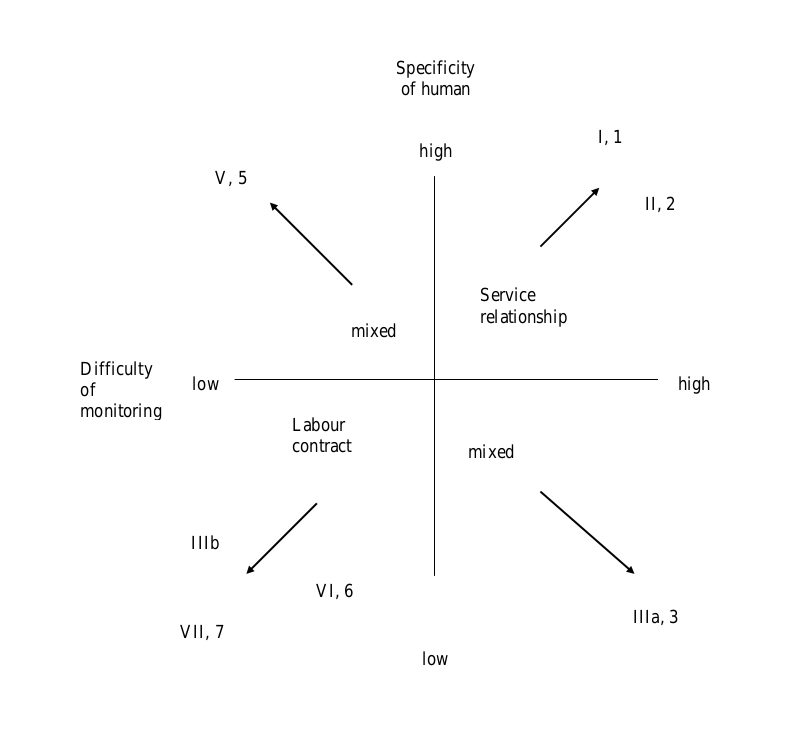
\includegraphics[width=\textwidth]{fig/Goldthorpe_ansaettelseskontrakt.png}
	\caption{Dimensioner af ansættelseskontrakten i Goldthorpes klasseskema}
	\label{fig_teori_klasse_Goldthorpe_arbejdskontraktdimensioner}
\end{centering}
\end{figure}

Den vertikale akse er specificiteten af kompetencerne, og kræver ikke yderligere forklaringen end den allerede givne.

Den horisontale akse, derimod, er udtryk for kontrollen over arbejdsprocessen. På venstre side er arbejdet af en sådan karakter, at dets udførsel og produktivitet let overvåges. Typisk vil det være manuelt arbejde.   
Til højre side findes arbejde, hvis karakter gør det svært at overvåge, og som ofte er service- relateret, eller har en symbolsk karakter, hvilket gør dets værdi og udførsel sværere at vurdere og overvåge. 

Det ses, at i det nederste venstre kvadrat gør kombinationen af højt udbud af færdigheder og nem monitorering en bestemt ansættelseskontrakt oplagt, \emph{arbejdskontrakten}. Det betyder at ansættelseskontrakten tilnærmer sig arbejdskraft som ren vare, da det er muligt at bestemme dens værdi ganske nøjagtigt. Dette er naturligvis den optimale situation set ud fra en arbejdsgivers synspunkt, og vil ofte indebære timelønning eller akkordlønning. Dette er arbejderklassens lod på arbejdsmarkedet. % skriv mere her når du gider, fx det med korter fyringsvarsler, mere som arbejdskraft man køber og sælger når man har brug for det. FX kan man se på skemaet at det der adskiller klasse IIIa og IIIb er at det er svært at overvåge arbejdet, men det er rutinepræget på en sådan vis at det er lige uspecifikt i kompetencer. Så grunden til at IIIa er så højt, er argumentet, at det er svært at overvåge deres arbejde.

I øverste højre kvadrat findes hvad Goldthorpe kalder ansættelseskontrakt som \emph{servicerelation}. De specifikke færdigheder giver gode muligheder for at forhandle gunstige arbejdsvilkår, og den diffuse målbarhed  kræver en incitatementsstrukturer, så lønmodtageren føler sig ansvarlig for firmaets mål. Dette er hvad hvad Goldthorpe kalder serviceklassen, eller \emph{salariatet}%
%
\footnote{Det kan være fornuftigt at benytte termet salariat fremfor serviceklasse, da det sidste kan forveksles med den slags repetitivt servicebaseret arbejde, der findes i dele af arbejderklassen og den lavere del af middelklassen, hvilket ikke er meningen: Salariatet er de to lønmodtagerklasser, der er \emph{mest} økonomisk begunstigede.}%
%
 \parencite[22]{GoldthorpeMcKnight2004}. %skriv mere når du gider hvis du gider at du gider

I disse to kvadrater kan man altså tale om, at selve arbejdets karakter giver enten arbejdsgiver eller arbejdstager fordele i forhandling af ansættelseskontrakten. I de to øvrige kvadrater er der tale et et blandet magtforhold, og der vil derfor være tale om et miks mellem de to typer ansættelseskontrakter. 

Ud fra disse to diffenteringsprincipper, baseret på bestemte arbejdsvilkår,laver Goldthorpe et klasseskema med 11 kategorier. Det er ud fra disse principper for arbejdsdelingen, der er grundlaget for magtpositioner, som de kommer til udtryk i ansættelseskontrakten. Ud fra disse udgår den sociale relation, en given arbejdstager har til produktionsmidlerne. % når analysen af Goldthorpes klasseskema er lavet med moneca, vurder hvor meget du skal skrive om hans klasseskema specifikt. FX det også kan kollapes til færre.


\label{klasse egp11}



Man kan sammenfatte Goldthorpes forståelse af hvad klasse \emph{gør} på følgende vis: 
%
\begin{enumerate}
 \itemsep-0.3em 		
 	\item Forskellige begivenheder indtræffer med forskellig styrker alt efter klasseposition
 	\item Forskel i interessedrejning hos forskellige klasser
 	\item Omkostninger forbundet med at forfølge en given interesse
\end{enumerate}
%
(Goldthorpe i \parencite[93]{Harrits2014}). Goldthorpe ser klassehandlen som  udtryk for de rationelle handlinger, et individ i en bestemt situation vil være tilbøjelig til at træffe. En rationel handlen defineres ud fra de økonomiske omstændigheder, individerne befinder sig i. I Goldthorpes fortolkning af økonomiske omstændigheder, vil det sige forholdet til produktionsmidlerne. Goldthorpe trækker på nymarxisten Jon Elsters forståelse af klassebaseret handlen som rationelle kollektive handling: Forskelle i belønninger kontra risici kan forklares ud fra sammenlignelige ressourcer i bestemte typer job. Især to forhold: Forskelle i begivenheder, der indtræder med forskellig styrke for forskellige klasser, fx arbejdsløshed, leder til \emph{ens}, men ikke nødvendigvis \emph{fælles}, handlingsmønstre indenfor klassen. individer i arbejderklassen have større risiko for arbejdsløshed, hvilket har betydning for den økonomiske sikkerhed, der findes i tilværelsen. Et andet eksempel er den økonomiske stabilitet, man kan forvente: i hvor høj grad et individ kan regne med, at lønindkomst er forudsigelig fra år til år, eller måned fra til måned, endda fra uge til uge \parencite[6, 10]{GoldthorpeMcKnight2004}.

Det andet: de transaktionsomkostninger og risici, der er forbundet med at forfølge bestemte mål, vil være ens, hvilket vil påvirke adfærd for individer i samme klassesituation. Børn fra mindre privilligerede familier vil have tendens til at satse på erhvervsrettede, kortere uddannelser, da afkastet i en sådan livsinvestering ikke kræver en risikabelt høj indsats, og sandsynligheden for en succesfuld sikring af klasseposition er høj, i deres position. 

Disse økonomiske forhold udgør en økonomisk virkelighed, som er ens for individer i samme klasseposition. Goldthorpe mener, at der i disse sammenhænge findes økonomisk rationelle strategier, som individer derfor vil have tilbøjelighed til at agere efter. Her understreger han, at i en given klassehandlen - altså kollektiv organisering for en gruppe lønmodtagere - kan det meget vel være mere rationelt at søge en korporativistisk fremfor antagonistisk strategi \parencite[215]{Goldthorpe2002}. Goldthorpe er ikke marxist, hvilket også ses i den forstand at han ikke anser \emph{en bestemt} type politisk handling som den objektivt rationelle, hvilket RAT-orienterede marxister har for vane at gøre (find henvisning til Boehmer, Wright, og ham fra Norge whats-his-face \#todo). Den danske velfærdsstatsmodel er eksempel på dette, hvor fagforeninger har anset det som mere fornuftigt at forfølge en overordnet korporativistisk strategi gennem det 20. århundrede. % referer til den der DSS bog? \#todo
% (Harris s. 93, hun citerer Goldthorpe 2000, find den og læs det (sociology and numbers hedder det vist, find det) \#todo

Overgang kunne være Oesch der citerer Goldthorpe for at se disse trends, men ikke mene at de er betydningsfulde endnu. (Oesch s. 28)


%%%%%%%%%%%%%%%%%%%%%%%%%%%%%%%%%%%%%%%%%%%%%%
\section{Daniel Oesch og arbejdslogik  \label{sec_}}
%%%%%%%%%%%%%%%%%%%%%%%%%%%%%%%%%%%%%%%%%%%%%%

Daniel Oesch er en schewizisk sociolog, der har søgt at reformulere et nyt grundlag for et klasseklassifikationsskema. Som hos Goldthorpe er udgangspunktet for klassedelingenden sociale relation til produktionsmidlerne, operationaliseret til erhvervsbeskæftigelse. 


Oesch mener at der sket så væsentlige ændringer i klassestrukturen, siden de mest benyttede klassifikationsskemaer blev lavet i 70'erne og 80'erne, af Wright og Goldthorpe. Denne periode var slutningen på hvad han kalder kapitalismens “gyldne æra,” og indfanger ikke klassestrukturen, som udviklingen har ført med sig, til et samfund delvist baseret på “postindustriel” produktion. Til forskel fra Daniel Bell (reference her \#todo), der forudså udviklingen af et postindustrielle samfund som en positivt betonet rationalisering og meritokratisering af samfundet, der førte til en opløsning af klassesamfundet, antager Oesch ikke en sådan udvikling. For Oesch betyder udviklingen af en offentlig sektor, kvindernes indtog på arbejdsmarkedet og  væksten i antallet af servicejobs, at klassekompositionen har \emph{ændret} sig, ikke opløst sig. Det er denne ændring, han vil indfange med sit klassifikationskema.  

Den bredere historiske analyse af årsagerne til denne ændring springer jeg let henover.

Man kan sige meget om årsagerne til disse udviklinger: Tænkere som Deleuze, Baumann, Adorno, (ham med netværkssamfundet), Negri \& Hardt, Richard Florida, Peter Wagner, Bourdieu m.m.fl. har forsøgt dette i mange år. Her vil jeg først redegøre for de tre tendenser, Oesch ser som væsentlige for at forstå ændringen i klassestrukturen. Dette sker kortfattet og hver tendens for sig. Derefter vil jeg gå lidt mere i dybden og forklare, hvordan samspillet mellem disse tre kommer til udtryk i en ændret klassestruktur, og hvordan Oesch mener at indfange denne struktur i sit klassifikationsskema. 

%
\subsection{årsager til ændringer i klassekompositionen \label{  subsec teori klasse Oesch aarsager}}
%


%
\subsubsection{tre årsager}
%


% industri- og serviceerhverv vækst findes der danske tal? \#todo

I forklaringen af den ændrede klassestruktur peger Oesch på 3 tendenser, der i perioden fra 70'erne og frem slog igennem i moderne vestlige samfund. Oesch viser udviklingen i disse tre tendenser, som de ser ud for Sverige, Tyskland, England og Schweiz \parencite[30]{Oesch2006a}.

Den første tendens er at den tertiære sektor/servicesektoren er vokset. Det betyder ikke kun flere jobs med høj specialiseret faglighed, det betyder også en vækst i antallet af servicefag med relativt lave uddannelseskrav. med andre ord sker er der sket en betydelig differentiering ud i forskellige typer af ikke-manuelle jobs. Dette ændrer på forholdet mellem manuelt/ikke-manuelt arbejde, hvor ikke-manuelt arbejde ofte automatisk har indebåret bedre vilkår end manuelt arbejde. Det mener Oesch ikke længere er tilfældet, og dette har ændret selve klassestrukturen \parencite[47]{Oesch2006a}. 

Den anden tendens er kvindernes indtræden på arbejdsmarkedet. I sin diskussion af Goldthorpes skema citerer Oesch Goldthorpe for at vedstå sig, at mange kvinder netop befinder sig i hans \texttt{klasse IIIb: lowergrade (hvad hedder det på dansk? find Harrits ord for det \#todo) rutinepræget ikke-manuelt arb.} \parencite[44]{Oesch2006a}. \texttt{Klasse III} benævnes samlet set som en slags “mellemposition”, eller middelklasse. Denne er karakteriseret ved at have en lav grad af “\emph{klassehed}” i sig; det vil sige, den fungerer som en slags residualkategori for serviceerhverv, der ikke har en høj status grundet uddannelsesmæssige specifikationer, eller i Goldthorpes jargon: sjældne kompetencer (det hedder det ikke men hvad hedder det så \#todo). Det er i høj grad kvinder, der fylder denne kategori, og Oesch mener at en nytænkning af klassifikationslogikken er nødvendig, for at tage højde for den permanente gruppe af servicebaseret, rutinepræget og primært \emph{kvindelig}, arbejdskraft, der er lokaliseret her \parencite[45]{Oesch2006a}. 

Den tredje tendens er ekspansionen og det generelt højere niveau af uddannet arbejdskraft. Det gælder også indenfor de traditionelt lavtuddannede - eller helt uuddannede - manuelle erhverv og de mange nye lavtløns jobs i servicesektoren. Det er især i de ikke-universitetsbaserede, erhvervsrettede serviceerhverv, at ekspansionen har været kraftig, ifølge Oesch (find henvisning \#todo)

Goldthorpe baserer sit skema på samfundet som det så ud i 70'erne, og siger selv, at hans formål ikke har været at forudsige tendenser i økonomien \parencite[48]{Oesch2006a}, men lave et klasseskema baseret på den nuværende økonomiske struktur. Oesch argument er, at disse tendenser ikke længere er tendenser, men \emph{er blevet} til den nuværende økonomiske struktur i (sen)moderne vestlige samfund. 

%
\subsubsection{Det ambigiøse i den automatiske hierarkisering af ikke-manuelt arbejde over manuelt}
%

For Oesch fører disse tre tendenser til en nuværende klassestruktur, hvor den traditionelle hierarkiske placering af ikke-manuelt arbejde over manuelt arbejde ikke længere er farbar; Det er ikke en hierarkisering, man kan tage for givet. Eller som Croutch siger det: “\emph{There are no grounds for regarindg the lower levels of the non-manual hierarchy as somehow superioer to manual work}” (ref \#todo) 1999:165. 

De lavtrangerende servicejobs inkluderer eksempelvis ikke den middelklassestatus, der ifølge Oesch tidligere var associaseret med ikke-manuelt arbejde. Disse servicefag har ofte en høj andel af kvinder, hvilket har betydning for deres placering på arbejdsmarkedet og dettes hierarki.   Sammenhængen mellem klassestrukturen og andre dybtliggende sociale strukturer såsom køn eller etnicitet bliver tydelig: Det er ikke et tilfælde, at arbejdsmarkedssegmenteringssteorien i USA er så optaget af den afroamerikanske befolknings placering på arbejdsmarkedet. Dette har ikke samme relevans i Danmark og andre nord- og vesteuropæiske lande%
%
\footnote{  I forbindelse med østudvidelsen af EU har vi set en diskussion af etnicitet særligt indenfor byggebranchen, restaurationsbranchen og rengøringsbranchen, og naturligvis også i diskussionen af indvandring fra ikke-vestlige lande. Min påstand vil dog være, at selvom dette påvirker visse brancher, og ikke er uvæsentligt, har det på ingen måde et omfang i Danmark, eller andre nord-og vesteuropæiske lande, der kræver en nytænkning af klassifikationslogikken som helhed. I modsætning til USA, hvor det forståeligt nok optog klasse-og arbejdsmarkedssegmenteringsteorietikere en hel del}%
%
. Det er muligt dette ændrer sig i fremtiden, og/eller allerede er på vej, som eksempelvis Mattias Tesfaye påpeger (henvisning \#todo). Kønsopdelingen af beskæftigelsesstrukturen og servicefagenes indlejring har dog en hel del flere år på bagen i de føromtalte samfund. Jeg vil formulere det således:
1) Den velkendte strukturelle placering af kvinders pligter/arbejdsområder under mænds i den traditionelle arbejdsdeling i hjemmet, gentages på arbejdsmarkedet i den samfundsmæssige arbejdsdeling, efterhånden som velfærdsstaten gradvist har overtagelet af en række af disse arbejdsopgaver op igennem den sidste halvdel af det 20. århundrede.2) Servicebaserede, rutineprægede erhverv såsom sekretær-relateret, adminstrativt arbejde, samt kundebetjening, har historisk set beskæftiget kvinder, og en vækst i efterspørgslen efter denne type jobs, bærer fortsat præg af dette. 

Det er ikke min - eller Oesch - påstand at dette udelukkende er kønsrelateret, og det er derfor jeg laver ovenstående skelnen mellem  traditionelt husarbejde og traditionelt servicearbejde. Det bliver interessant at se på, om eller hvorledes dette gør sig gældende på det danske arbejdsmarked. 

Nøglen er, ifølge Oesch, at lave en teoretisk konsistent klassifikation, således at skellet mellem manuelt/ikke-manuelt arbejde ikke per automatik medfører en vertikal placering af det sidste over det første. Dette skift i klassesstrukturen vil man have tilbøjelighed til at overse, hvis man benytter \emph{husstanden} som observationsenhed for klasseposition. Dette er ikke i sig selv en fejl, det kommer an på hvad der skal undersøges; Mere om det i afsnit REF \#todo. Men eftersom man i disse undersøgelser tit har taget mandens klasseposition som mål for husstanden, ser man, ifølge Oesch, ikke det føromtalte skift i klassestrukturen klart, da mandlige beskæftigede i langt højere grad stadig følger den vertikale placering af manuelt arbejde under ikke-manuelt arbejde \parencite[42]{Oesch2006a}.

Denne ambiguitet mellem “håndens og åndens” arbejde skyldes ikke kun væksten i antallet af rutineprægede servicejobs, men hænger sammen med en uddannelsesmæssig opgradering, også af den industrielle arbejdsstyrke. Denne opgradering har betydning både i toppen og bunden af arbejdsmarkedet: I bunden af arbejdsmarkedet
%find henvisning til snak om "den fjerde industrielle revolution"
reducerer uddannelsesvæksten/inflationen den sociale afstand mellem “bluecollar” \emph{arbejdere} og “whitecollar” \emph{ansatte(?!?)} . Distinktionen mellem arbejder og ansat er blevet mindre markerede, peger flere undersøgelser på \parencite[49]{Oesch2006a}. 

I toppen af arbejdsmarkedet kritiserer Oesch Goldthorpe for at betragte servicekontrakten til arbejdsgiveren som et homogent udtryk for \emph{én forenet} horisontal position indenfor serviceklassen%
%
\footnote{ Kun horisontalt, ikke vertikalt: Som beskrevet på side \pageref{klasse egp11} opdeler Goldthorpe selv serviceklassen i forhold til specifiteten af kompetencer, i en øvre og en nede serviceklasse.}%
%
 Goldthorpe insisterer på denne horisontalte enhed i serviceklassen, da han ingen teoretisk konsistent begrundelse har for en horisontal distinktion. Det kritiseres af Oesch for at være \emph{“somewhat academic”} \parencite[53]{Oesch2006a}. Med andre ord: Teoretisk stringens sættes højere end de differentieringer på arbejdsmarkedet, Oesch mener Goldthorpe dermed udelukker fra sit klasseskema.





 Denne forskel er på ingen måde så uskyldig som den lader til at være: faktisk åbner den netop den can of worms, som Oesch selv hævder han gerne vil lukke, når han fx siger han eksplicit vil betragte økonomiske klasser. Men det er jo netop det, Goldthorpe holder fast i her, og som Oesch så alligevel ikke mener er tilstrækkeligt. Det er ikke nødvendigvis et dårligt argument for uholdbarheden af rene økonomiske klasser, desværre præsenteres det ikke sådan af Oesch, der tværtimod - måske uden helt at være klar over det, eller ihvertfald uden at drage konsekvenserne vidtrækkende nok - først vil holde sig udelukkende til økonomiske klasser, men her reelt bryder med netop dette. Og, ironisk nok, uden at omtale det sådan, kritiserer Goldthorpe for netop at holde sig \emph{indenfor} de grænser, han selv siger må være horisonten for et udelukkende arbejdsmarkedsorienteret klasseskema! 






 Dette skyldes at Goldthorpe ikke vil 


ifølge Oesch, for at 



For det tredje er det tidligere omtalt \emph{salariat} øget i såvel antal som i heterogenitet. Det gælder både hvad Oesch kalder de management-lignende beskæftigelser samt de mere klassiske professioner%
%
\footnote{Professionerne skal her forstås i samme forstand som hos Goldthorpe på s. \ref{professionerne_def} \#todo}%
%
. De tre nævnte effekter i form af højere uddannelse%
%
\footnote{Eller,  med dansk uddannelsesforsknings \emph{grand old man}, Erik Jørgen Hansen, uddannelses\emph{inflation} find henvisning fra dds \#todo}%
%
, vækst i den tertiære sektor samt udviklingen af den offentlige sektor har haft en effekt inden for sammensætningen af disse middelklasser, omend - naturligvis - med andre effekter end på de andre to typer klasser. I væksten af velfærdsstaten ser Oesch det eksempelvis ikke køn som en central akse, som han gør det i de lavere serviceerhverv \parencite[2f]{Oesch2006a}. 
Denne forskel i betydning af det offentliges vækst for henholdvis de lavere servicefag og salariatet, argumenteres der ikke direkte for. Mellem linjerne kunne man sige at der ikke er tale om traditionelt kvindearbejde 

Resultatet er en klassestruktur, hvor sammenhænge mellem politiske holdninger, livsstil og økonomi har en anden dynamik end tidligere, hvilket alle klasseteoretikere mig bekendt anerkender (se Scott, Grusky, Harrits, Carsten etc etc find henvisninger \#todo). Eksempelvis gør salariatets heterogenisering det umuligt at behandle som en monolitisk størrelse, under een betegnelse såsom \emph{middelklassen}, eller evt. todelt til \emph{højere} og \emph{lavere} middelklasse, som vi ser hos Goldthorpe. Selvom Goldthorpe, som beskrevet på s ?? (\#todo) har yderligere opdelinger, er Oesch ikke overbevist om at dette er tilstrækkeligt for at forstå hvor forskellige de positioner, salariatet optager, egentligt er. Han mener der kræves ikke bare en \emph{empirisk} findeling, men en \emph{teoretisk} nytænkning af klassestrukturens diffenteringsakser i disse senmoderne, delvist postindustrielle samfund. 

\iffalse
\label{iffalse}

Oesch minimale klassedefinition: similarity in the position within the occupational system \parencite[16]{Oesch2006a}
 	→ AHA! men hvordan defineres position! Jeg har et bud hehehehe og det er anderledes end Oeschs hehehehe.

Breen: The major origin of data of class still rest on the golden age of capitalism  (oesch 1996, 16), s1 (nederst)

Økonomisk klasse: deler latente interesser i form af ens økonomisk situation, og ikke nødvendigvis meget andet. I modsætning til social klasse, der har større krav til identitet og ens organisering.  sæt evt. bourdieu what makes a class ind i den diskussion, for at kunne skille tingene ad. . wuhuu det blir godt. Eller Scotts distinktion mellem "social class" - household etc, og så klasseposition - individets klasseposition (refer til Scott 1994 ligesom Oesch gør det, s. 13)





klasse III i EGP består i høj grad af kvinder, og har i sin "intermediateness" et problem - måske er vi kommet langt nok i udviklingen af dette som en fast bestanddel til at kunne dekomposisere den? Lavet om til IIIb og IIIa netop af denne grund. Men er det nok? s. 46 vist nok

manual/non-manual ser ikke ud til at være brugbart rent hierarkisk s. 47-8. Ellers noget man har gået meget op i med fx. Lukacs. Darhendorff ser ud til at være mere brugbar

Bourdieu ser ikke ud til at være den bedste til at forstå det her ud fra. 

en udvidelse af en række jobs, hvilket man ser i jobs som s.49 - det finder jeg også!




Bruge arbejde eller markedssituation?
	→ klart reduktionistisk, me måske nødvendigt for at skabe sig et overblik. I dunno.

lav exceldata også på Oesch og Goldthorpes skema. Do it now!!! 




ps der er gratis kokain til de fem første!





artiklen om Trumps hvide arbejdervælgere. Brug den som argument for magten i klasseanalyse!


Goldthorpe laver, ligesom Weber, en skelnen mellem social klasse og social \emph{status}. Det 



s. 10 individuelle og strukturelle faktorer 



Det er ikke nødvendigvis sådan, at alle individer indenfor samme klasse forfølger samme interesser. Snarere sådan at individer i samme klasseposition vil have større affinitet overfor de samme interesser. Goldthorpe benytter Webers forståelse af social orden, forbundet med ære og hierarkisk værdisætning, som selvstændig kilde til social stratifikation og livsanskuelse. Disse værdisæt har ifølge Goldthorpe antaget en løsere form som det 20. århundrede skred frem, uden at det dog ser ud til at opløse dets effekter - snarere er denne form for “verdensanskuelse” langt mere betydningsfuld for at forstå eksempelvis kulturforbrug, og de politiske holdninger på en værdipolitisk akse, gående fra liberitær til autoritær (Goldthorpe i \parencite[95]{Harrits2014}. 

Selvom Goldthorpe understreger denne sociale status kilde til at forstå individerne og deres subjektivitet, er hans EGP-klasseskema dog strengt baseret på position på arbejdsmarkedet, da han laver denne skelnen mellem de to niveauer \parencite[95]{Harrits2014}. 








 









Det vil jeg gøre med følgende fremgangsmåde. 

Først vil jeg gennemgå Marx, der definerer relationerne til produktionsmidlerne som afgørende, og den udbytning, de danner basis for, og som definerer de sociale relationer. Derefter vil jeg gå ind i nymarxisternes hovedpine med basis-overbygningsmodellen, eftersom klassesamfundet ikke blev polariseret i to store klasser, sat imod hinanden, men i stedet fremkomsten af nye middelklasser samt nye serviceerhverv, der ikke ser ud til at være midlertige, men tværtimod helt nødvendige dele af den moderne kapitalisme. Jeg vil slutte min gennemgang af marxismens bud på stratifikation på arbejdsmarkedet ved det for mig at se mest empirisk anvendelige bud Eric Olin Wrights klassemodel.

Derefter vil jeg kort gennemgå Weber, der skelner mellem social status, klasse og stænder. Han har inspireret John Goldthorpes meget anvendte såkaldte EGP-klasseskema, der vil blive gennemgået som det næste, med dets fokus på kontrol over arbejdsprocessen og specifiteten af faglige kompetencer som de centrale differentieringsmekanismer. Goldthorpe har en analytisk-teoretisk funderet klasseforståelse, som bliver udfordret af David Grusky, der er fortaler for en noget anderledes klasseforståelse, baseret på erhvervsgrupper og de reelt oplevede fællesskaber, der findes her. Han benytter sig af Frank Parkins begreb om sociale lukningsmekanismer, som også bliver gennemgået (til Jens: sikkert for grundigt gennemgået, skal skæres til). I forhold til MONECA er hans bud spændende, da han udfordrer ideen om store klasser, og er fortaler for disse mikroklasser, som han mener drukner i de i sammenligning grovkornede klasseinddelinger, baseret på teoretiske principper. For mig at se kan Moneca netop være en måde at opdele i større klasser, baseret på empiriske bevægelsesmønstre, det vil sige give plads til Gruskys anke mod "big classes", som for mig at se er fornuftig nok, i og med en undersøgelse på mikroniveau kan afsløre klassedynamikker man ikke fanger på et højere plan. Jeg synes dog Gruskys teoretisk grundlag og affejning af teoretiske klasseinddelinger er problematisk, og hans afvisning af at der findes effekter af at tilhøre større klasser end erhvervsgrupper er problematisk. Her er Moneca en metode, der nærmest virker som skabt til at fungere på begge niveauer, det vil sige som beskrivelse af erhvervsgrupper på meget detaljeret niveua, samt mulighed for at afdække fællestræk i deres "sociale processer" på segmentniveau.

%til sidst vil jeg lede det over i metodeafsnittet, da både Grusky og Goldthorpe benytter økonometrisk funderet regressionsanalyse, og jeg vil mene at en relationelt funderet social netværksanalyse har mulighed for at klasser som relationelle størrelser, fremfor som udtryk for variable.



%DET VIL JEG VIL GØRE MED FØLGENDE FREMGANGSMÅDE...

% Forskellige bud på klasser
% 	Marx
% 		-forholdet til produktionsmidlerne, udbytning
% 	Nymarxisme	
% 		- Problemerne i basis-overbygning og middelklassens position
% 		- Redskaber mere nuancerede end kapital-arbejde - hvordan, og stadig beholde den marxistiske kerne? 
% 	Wright
% 		- klasse som forklarende og nominel (tror jeg)
% 		- Tre dimensioner: Ejerskab over produktionsmidler, autoritet, færdigheder
% 	Weber
% 		- Klasse, social status og stænder
% 	Goldthorpe
% 		- Klasse som forklarende og nominel
% 		- Tre dimensioner: Ejerskab over produktionsmidlerne (knapt så centralt), specifiteten af kompetencer, kontrol over arbejdsprocessen 
% 	Grusky
% 		- Klasse som beskrivende og realistisk
% 		- kritik af nominel klasseinddeling
% 			- for grovkornet
% 			- misser det centrale ved definition udenfor de reelt oplevede fælleskaber
% 		- erhvervsgrupper som klasser, sociale lukningsmekanismer

%DET SKAL ALT SAMMEN BRUGES TIL...

	% Opsamling: 
	% 	- Kobling til delanalyse 1: Moneca som måde at inddele arbejdsmarkedet i segmenter (klasser)
	% 	- Kobling til delanalyse 2: Forklare sociale processer i segmenter (klasser) vha. klasseforskere
	% 	- Kobling til delanalyse 3: Jeg  placere Moneca som et oplagt bud på at mediere og vurdere de to positioner (den realistiske og nominelle klasseindling)

Denne teoretiske gennemgang skal bruges til følgende i forbindelse med det overordnede spørgsmål om arbejdsmarkedets segmentering, i 3 analyser:

\begin{itemize}
  \item Delanalyse 1: Moneca som måde at inddele arbejdsmarkedet i segmenter
  \item Delanalyse 2: Forklare sociale processer i segmenter (klasser) vha. klasseforskere
  \item Delanalyse 3: Moneca som på at mediere og vurdere de to positioner (den realistiske og nominelle klasseindeling hos henholdsvis Grusky og Goldthorpe)
\end{itemize}



%Motivation for at inddrage klasseteori er, at analysen af delmarkeder/segmenter og mobilitet ligger inden for en tradition af klasseteori. Dette ses såvel i Wrights analyse/teori om bla bla bla såvel som i Gruskys analyse/teori om...

%Arbejdsmarkedssegmenteringsteorien, som ligger til grund for Toubøl, Larsen og Strøbys udvikling af en a posteori arbejdsmarkedssegmenteringsanalyse, ligger inden for en amerikansk/anglo-saksisk økonomisk diskussion op i mod den neoklassiske økonomiske teori \parencite[2]{Touboel2013}. Thomas Boje opsummerer kritikkken således:

%\begin{displayquote} “\textit{The core of this criticism is first that neoclassical labour-market theories in their analogies to the commodity market do not take into account the heterogeneous character of the labour market and the lack of homogeneity in the labour force. Secondly the theories do not take into account that the behaviour of individuals on the labour market is not governed by economic utility maximization, but, on the contrary, determined by social relations and institutions of which the individual is an integral part.}” \parencite[171]{Boje1986}. \end{displayquote}

%Segmenteringsteorien fremkomst primært i USA opstod ifølge Cain i 1960'erne og 1970'erne som en reaktion på kampen mod fattigdom og fuld deltagelse i økonomien for blandt andet minoritetsgrupper og kvinder \parencite[1216]{Cain1976}. Doeringer og Piore opdelte arbejdsmarkedet i primære og sekundære markeder med “gode” jobs og sidstnævnte indeholder alle de “dårlige” jobs med henblik på at forklare den ulige fordeling af lønninger \parencite[70]{Doeringer1971}, mens Reich, Gordan og Edwards mere radikale tilgang tilgang beskrev, hvordan den historiske proces, hvorved politisk-økonomiske kræfter fremmer opdelingen af arbejdsmarkedet i seperate delmarkeder \parencite[359]{Reich1973}. Hvor denne segmenteringsteori tager udgangspunkt i forandringerne i sin tid og en økomisk kritik af økonomien, så er mit udgangspunkt og fokus et andet. Mit udgangspunkt er den sociologiske tradition, klasseteori og klassediskussion.

%Derfor vil jeg frem for at dykke ned i segmenteringsteoretikerne tage fat i de sociologiske klaseteoretikere såsom Marx, Weber, Gitte Harrits, Goldthorpe, Wright, Parkin og Grusky. Disse teoretikere er både med til at forklare det første kritikere i forhold til delmarkeder og mobilitet (fx Weber og Goldthorpe), hvilket var bla bla bla... Samtidig ligger der også inden for andet kriterie det vil sige, hvorfor der er forskellen på et delmarked og et segmenter er forskelle i sociale processeser (fx Wright og Goldthorpe). Alt sammen er det interessant også for det tredjhe kriterie oim hvorfor sociale processer fører til segmentering.




%%%%%%%%%%%%%%%%%%%%%%%%%%%%%%%%%%%%%%%%%%%%%%
\section{Karl Marx \label{2_marx}}
%%%%%%%%%%%%%%%%%%%%%%%%%%%%%%%%%%%%%%%%%%%%%%

Marx selv nåede aldrig at færdiggøre sin klasseteori, eller skitsere den i en sammenhængende form. Kapitel 52 i tredje bind af \emph{Kapitalen} har titlen "Klasserne", men efter cirka en side stopper skriften, og Engels, der udgav værket efter Marx' død, skriver: "Her afbrydes manuskriptet" \parencite[22]{Harrits2014}. Som samlet klasseteori må man derfor benytte sig af Marx' generelle teoriapparat, for at forstå hvad en klasse er hos Marx. Det er værd at huske på, at netop fordi klasserne ikke nåede at modtage en specifik teoretisk behandling, må klasseteorien konstrueres ud fra hans generelle historieforståelse.

Formålet her er ikke en grundig gennemgang, men en skitsering, der skal tydeliggøre fundamentet i den neomarxistiske klasseforståelse.

Klasserne hos Marx er defineret ud fra den tilgang, at det vigtigste menneskelige forhold omhandler produktionen af livsfornødenheder, altså de materielle forhold. De værktøjer - forstået i bredest mulige forstand - som gør det muligt at producere disse livsfornødenheder, defineres som produktionsmidlerne. Menneskers forhold til produktionsmidlerne er dermed den centrale sociale relation i et samfund, og igennem denne primære sociale relatio udgår alle andre sociale relationer. Det vil sige, at mennesker med samme sociale relation, lad os kalde det ejerskabsforhold, til produktionsmidlerne, kan karakteriseres som en klasse, da de deler det mest centrale grundvilkår, nemlig betingelsen der tillader dem at reproducere deres livsgrundlag. Marx peger på det forhold, at mennesker er i stand til at arbejde mere, end det der skal til for at holde dem i live, og det arbejde, der ligger udover hvad der skal til for at reproducere dem som arbejdskraft, kaldes merarbejdet. Det er dette arbejde, der er grundlag for udbytningsrelationer mellem forskellige klasser, hvor nogle klasser i kraft af deres ejerskab over produktionsmidlerne kan nyde godt af de primære producenters arbejdskraft. Det er således både en dominansrelation og en udbytningsrelation på spil, i forholdet mellem de eller den herskende klasse og den eller de klasser, der tvinges til at arbejde for dem.

Kapitalistiske samfund er kort sagt karakteriseret ved, at penge bliver den centrale mediator mellem forskellige former for arbejde. Hvad enten den er indlejret som arbejdstid i en fysisk form som en stol, et kilo sukker, eller i et menneske, som levende arbejdskraft. Det er denne "universelle ækvivalent", som Marx kalder den, der tillader det moderne kapitalistiske marked, hvori alle former for menneskeligt arbejde kan udveksles frit som varer. Frit er det dog ikke helt, da det er Marx påstand, at kun en enkelt vare rummer en ganske særlig kvalitet, nemlig evnen til at avle mere arbejde end det, der er indlejret i den. Den vare er mennesket. Et kapitalistiske samfund er derved karakteriseret ved lønarbejde, hvori en klasse, borgerskabet, ejer produktionsmidlerne, mens størstedelen fungerer som den arbejderklasse, der bliver betalt mindre, end deres arbejde er værd, men nok til at reproducere deres arbejdskraft. Det er Marx forudsigelse, at i overgangen fra feudalsamfundet til det kapitalistiske samfund, vil størstedelen af feudalsamfundets udbyttede klasser blive tvunget fra at have, eller i det mindste være i besiddelse af, deres egne produktionsmidler, til at arbejde direkte for borgerskabet i form af løn. Det kapitalistiske samfund vil derfor blive karakteriseret ved en tiltagende polariseret klassekamp mellem arbejdere og kapitalister, bourgeosi og proletariat.

Det behøver ikke nødvendigvis tolkes sådan, at der findes to klasser, der empirisk stringent kan deles op, selvom det, særligt i mere polemisk og politiske øjemed, er blevet benyttet sådan. I Marx' egne konkrete klasseanalyser benytter han en række termer for klasser og klassefraktioner, ikke kun bourgeosiet og proletariatet. Snarere er påstanden, at der findes en grundlæggende modsætning mellem arbejde og kapital, og denne modsætning er afgørende for interesserne og handlemønstrene for dem, der står på henholdsvis den ene og den anden side af denne modsætning. Her benytter Marx sig af begreberne "klasse i sig" og "klasse for sig", hvor det første er en klasse, der findes objektivt, bestemt af de sociale relationer, og det andet er en klasse, der forstår sig selv som klasse. Der er altså to niveauer i en klasseanalyse:

- et abstrakt niveau, der handler om kampen om merværdi og den grundlæggende klassemodsætning i samfundet
- et konkret niveau, om de observerbare klassefraktioner og grupperinger, der indgår i de politiske kampe i samfundet \parencite[26]{Harrits2014}. %lav til liste

Marx' teori indeholder derfor, som Harris fremhæver, ikke nødvendigvis en påstand om arbejderklassens enhed, men kan ligeså vel tolkes som en invitation til at lave historiske analyser med fokus på samfundsforandring, klassedannelse og politiske magtkampe \parencite[28]{Harrits2014}. I den marxistiske tradition ligger der altså et fokus på at bestemme klasser ud fra deres forhold til produktionsmidlerne, sagt med lidt mere almindelige termer: Hvilken overordnet beskæftigelse, man er i. Den fokuserer derfor på relationer indenfor produktionen, og ikke markedsrelationer, med særligt fokus på den \emph{udbytning} der findes i disse relationer.


%%%%%%%%%%%%%%%%%%%%%%%%%%%%%%%%%%%%%%%%%%%%%%
\section{Problemet med middelklassen og det marxistiske svar \label{2_nymarxisme}}
%%%%%%%%%%%%%%%%%%%%%%%%%%%%%%%%%%%%%%%%%%%%%%

Ikke desto mindre udviklede de moderne samfund sig ikke sådan, at kapitalismens centrifugalkræfter delte samfundet i to, med kapitalister og arbejdere sat overfor hinanden, grundet deres ensartede relation til produktionsmidlerne, som besiddende og ikke-besiddende. Den basale to-klasse model synes ikke at fange de interessemodsætninger og klasseformationer, som opstod i stabile kapitalistiske samfund. En række klasser i det sociale stratum med ejerskab over egne produktionsmidler, såsom artians, small traders, shopkeepers and småbønder, %hvordan fanden oversætter man det
forsvandt godt nok (evt. Parkin henvisning). Men denne polarisering i den socioøkonomiske struktur - altså en koncentration af produktionsmidlerne i færre hænder - blev historisk ikke til to store klasser, sat i mod hinanden, og den teoretiske skillelinje fra den marxistiske politiske økonomi mellem arbejde - kapital kunne tydeligvis ikke omsættes til en tilsvarende opdeling i klasser med egentlig ageren efter denne opdeling. Det vigtige i denne afhandling er, at selvom denne modsætning mellem arbejde - kapital måske nok findes - som påvist af bl.a. Thomas Pikkety, og strukturerer indkomstfordeling på afgørende vis, fungerer denne grundlæggende struktur ikke på nogen entydig måde, der gør denne opdeling særlig brugbar til at undersøge de klasseformationer, vi kan observere empirisk. 

En række andre forhold må medtænkes, da det er tydeligt at middelklassen, der erstattede det gamle småborgerskab, ikke er ekstern i forhold til den kapitalistiske produktionsmåde, men er en central del af den, som Parkin påpeger i sit værk \emph{Marxism and Class Theory: A Bourgeois Critique} fra 1979 \parencite[16]{Parkin1979}. %kan man henvise bare til siden når værket allerede er nævnt?

Der må altså være en række forhold, der muliggør eksistensen af den langt mere komplekse klassestruktur i senmoderne, stabile, kapitalistiske samfund, og som er af central betydning for at forstå klasseformationerne i dette.

Hvis arbejde-kapital ikke er en skillelinje, der giver særlig meget forklaringskraft i de samfund, der findes, hvad gør man så, for at finde de politisk relevante brudflader mellem klasserne? Og hvad skal man gøre med den føromtalte middelklasse? Det er hvad Parkin kalder \emph{the boundary problem in Marxism and sociology} \parencite[11]{Parkin1979}. 

Parkin identificerer tre nymarxistiske svar på dette problem. De to første skal kun kort skitseres, mens den sidste, repræsenteret ved Eric Olin Wright, bliver gennemgået i dybden. 

Det første svar er, hvad Parkin kalder \emph{den minimalistiske} definition af arbejderklassen, repræsenteret ved Poulantzas. Her drages skillelinjen mellem produktivt og uproduktivt arbejde, baseret på en fortolkning af hvilken form for arbejde, der skaber merværdi. Lønarbejde, der ikke skaber merværdi, er også udbytning, og indgår derfor ikke i proletariatet, altså den politisk relevante samfundsgruppe i marxistisk optik. Det giver en forklaring på stabile udbytningsrelationer, også lønarbejdere i mellem. 

Det andet svar er den \emph{maksimalistiske} version, repræsenteret ved Poul Baran, der benytter sig af Marx' lighedstegn, visser steder i sine skrifter, mellem \emph{folket} og arbejderklassen. De mange mod de få. Her benyttes et politisk defineret kriterie baseret på hvilke sociale grupper, hvis sociale funktion også ville være nødvendige i et socialistisk samfund \parencite[20]{Parkin1979}. Det er politisk i den forstand, at det handler om at skabe forening mod en overklasse, og analytisk i den forstand, at det prøver at forudsige, hvilket arbejde der kan siges at være \emph{samfundsmæssigt nødvendigt}, for på den måde at klassificere dem, der lever af andres arbejde.  

Begge disse svar forekommer mig ikke særlig anvendelige i en konkret klasseanalyse, og nævnes derfor kun som forsøg på at løse “\emph{the problem of the middle-classes}”, som som Wright kalder det \parencite[15]{Wright2000}. I stedet vil jeg fokusere på den nymarxistiske retning Parkin kalder \emph{mellempositionen}, som Parkin karakteriserer ved Erik Olin Wright selv \parencite[17]{Parkin1979}.


%%%%%%%%%%%%%%%%%%%%%%%%%%%%%%%%%%%%%%%%%%%%%%
\section{Erik Olin Wright \label{2_wright}}
%%%%%%%%%%%%%%%%%%%%%%%%%%%%%%%%%%%%%%%%%%%%%%

Erik Olin Wright introducerer to dimensioner for at forstå hvad han kalder \emph{modsætningsfyldte klassepositioner}, normalt omtalt som middelklassen: “\emph{people who do not own their own means of production, who sell their labor power on a labor market, and yet do not seem part of the working class.}” \parencite[15]{Wright2000}. Det giver samtidig anledning til at differentiere arbejderklassen og klassesamfundet generelt, i en mere nuanceret klassebaseret stratifikationsteori, der viser \emph{hvad klasse gør}, som Harris formulerede det. 

Centralt står stadig forholdet til produktionsmidlerne og de udbytningsrelationer, der hersker mellem mennesker, alt efter deres relation til produktionsmidlerne. Wright sætter to dimensioner på udbytningsforholdet, der udtrykker mulighederne for at tilegnelse af samfundets ressourcer. Klassepositioner ses som udtryk for en kombination af disse to akser samtidig med, at han bibeholder overordnede skelnen mellem ejer-ikke ejer.

Den første akse kalder Wright \emph{autoritetspositioner}, og omhandler det forhold, at kapitalejere uddelegerer deres lovmæssige ret til at lede og fordele arbejdet til andre. Det sætter dem i en modsætningsfyldt klasseposition, da de ikke er kapitalister selv, men står over arbejderne, og modtager højere løn for deres ansvar i en virksomheds daglige ledelse. Den anden akse kalder Wright \emph{færdigheder}, der beskriver de faglige og tekniske færdigheder, der er nødvendige for en given produktion. 



 % Søren: Dette kan bruges i forhold til sociale processer i segmenterne på sammen måde som "socia closure".


Udover disse akser har Wright, traditionen tro fra Marx, en skillelinje mellem ejere og ansatte, altså de, der selv ejer produktionsmidler, og de, der ikke gør. Disse to akser demonstrerer dermed en skala af klassepositioner, der muliggør forskellige slags tilhørsforhold og identiter, der ikke nødvendigvis polariseres i den enkeltdimensionerede arbejder-kapitalist relation, omend denne grundlæggende modsætning bibeholdes i modellen. Middelklassen bliver dermed den gruppe mennesker, der befinder sig i disse mellempositioner, og Wrights model muliggør også at positionere ansatte indenfor service- og informations industrien, der traditionelt har voldt marxistiske teoretikere en del genvordigheder.

Wright benytter denne udbyggede model til at forstå, hvordan man på det samfundsmæssige plan ser bestemte klasseformationer og politiske kampe, der gerne skulle kunne forklares ud fra denne klassemodel. Spørgsmålet om hvorvidt man skal kortlægge klassestrukturerer “bag om ryggen” på individerne står altså stadig centralt. Wright fastholder på den side ene side en teoretisk model, baseret på udbytningsrelationer i økonomien, samtidig med at den konkrete udformning af denne skal testes empirisk og revurderes løbende, baseret på dens evne til at forklare politiske kampe og observerede klasseformationer s. 75. 

% brug evt. henvisning fra Harris s. 67 til to konkrete danske analyser med brug af Wrights klassemodel 


%%%%%%%%%%%%%%%%%%%%%%%%%%%%%%%%%%%%%%%%%%%%%%
\section{Max Weber \label{2_weber}}
%%%%%%%%%%%%%%%%%%%%%%%%%%%%%%%%%%%%%%%%%%%%%%

Selvom Weber heller aldrig nåede at færdiggøre sin klasseteori, fremstår den i noget mere færdig form end tilfældet er hos Marx \parencite[28]{Harrits2014}. Webers klasseteori medtager stratifikation, der ligger udover hans klassebegreb, og indeholder derfor en mere pluralistisk tilgang til samfundets opdeling i forskellige sociale grupperinger. Hans klassebegreb er dog tydeligt inspireret af Marx, i den forstand at det er bundet op på økonomiske interesser og et bestemt forhold til produktionsmidlerne:
%
\begin{displayquote} “\textit{Vi vil tale om "klasse" når 1. livsbetingelserne for en flerhed af mennesker er betinget af en specifik fælles komponent, for så vidt 2. denne komponent ene og alene udgøres af økonomiske ejendoms- og erhvervsinteresser, og det foregår på 3. (vare- eller arbejds)markedets betingelser ("klassesituation"}” \parencite[302]{Weber1978}. \end{displayquote}
%
Til forskel fra Marx er klasser også defineret ved deres status på arbejdsmarkedet, fremfor relationen til produktionsmidlerne, og der ligger derfor et større fokus på markedsrelationer, altså “\emph{arten af éns chancer på markedet}” (weber 31 2003, i \parencite[29]{Harrits2014}). For at begribe disse chancer på markedet, der jo i høj grad er bestemt af hvilken økonomisk klasse, man er i, siger Weber, at det er ens evne til at tilegne sig indtægter og goder (Weber 1976 i \parencite[29]{Harrits2014}). Det åbner op for et kulturelt perspektiv, da alle mulige egenskaber, der kan omsættes til økonomiske ressourcer, bliver en del af et menneskes livschancer på markedet. Hos Weber finder vi et klassebegreb, der i udgangspunktet indeholder en typologi baseret på ejerskab/ikke-ejerskab over produktionsmidlerne, men derudover indeholder en langt bredere forståelse af klassefraktioner indkapslet i konceptualisering af hvad der definerer klasser. Og i øvrigt ligger tæt på Marx egne konkrete analyser af klasser, som omtalt tidligere.

Weber peger også på mobilitet mellem klasser som et centralt spørgsmål for klasseforskning. Så bevæger vi os hen til at beskrive, hvad klasse \emph{gør} parencite[302]{Weber1978}. Der er hos Weber et større fokus på den subjektive oplevelse af klassetilhørsforhold. Selvom folk individuelt reagerer ens på deres klassesituation, er det ikke ensbetydende med en deterministisk bevægelse hen imod en klasse-for-sig, som hos Marx. Weber er dermed mere interesseret i alle de aspekter, som en klasse \emph{gør}, fremfor Marx fokus på politiske kampe og social forandring. Klassebegrebet kan bruges generelt til undersøgelse af interessekampe, mobilitet og al mulig anden adfærd. (Harris 31). % Søren: Dette skal du vende tilbage til i analysen - intern mobilitet som en weberiansk klasse-/segmentopdeling.

Det sidste centrale begreb hos Weber er hans begreb om stænder. Det vil sige hans forståelse af, at der udover en økonomisk orden, også er en social orden, "den måde hvorpå social ære" fordeler sig i et fælleskab" (Harris 31). Denne sociale orden er en \emph{selvstændig} kilde til magt i et fælleskab, hvilket er en væsentlig forskel fra den marxistiske klasseanalyse. Det er knyttet op på subjektive oplevelser af fælleskab og anerkendelse af bestemte former for livsførsel om særligt attråværdige. Selvom Weber understreger stænders selvstændighed i forhold til klassesituationen, bliver spørgsmålet om sammenfaldet mellem klasse og stænder, og den måde, de kommer til udtryk på i en bestemt praksis, et genstandsfelt for klasseforskning \parencite[32]{Harrits2014}.




%%%%%%%%%%%%%%%%%%%%%%%%%%%%%%%%%%%%%%%%%%%%%%
\section{Grusky og Parkin \label{gruskyogparkin}}
%%%%%%%%%%%%%%%%%%%%%%%%%%%%%%%%%%%%%%%%%%%%%%

Grusky har to kritikker af klasseanalyse som den almindeligvis bedrives: For det første at de er nominelt funderede, fremfor at tage reelt oplevede, sociale fællesskaber som grundprincip for klasseinddelingerne. Og for det andet, at de derved ender med en grovkornet klasseinddeling, der skjuler udbytnings- og stratifikationsmekanismer, der burde være i centrum af klasseforskningen. 

%brug eventuelt: basis skal være institutionaliserede, "aktøroplevede" (dårligt ord) erhvervsgruppers i samfundet. Det er på dette niveau, at klasse reelt "fungerer" (Grusky 2001 eller 2002 find henvisning)

Grusky påpeger at menneskers identifikation med klassebaserede identiteter historisk er blevet svagere og svagere, samt den manglende massehandlen, der burde følge med positioner i arbejderklassen, hvilket har ledt til en hel del \emph{nymarxistisk håndvridning}, som han kalder det \parencite[205]{Grusky2001}. 

Det er ikke problemet at benytte beskæftigelse som grundlag for klasseinddeling. Problemet er niveauet af aggregering, der sker ved at placere en lang række forskellige professioner i eksempelvis kategorien \emph{nedre serviceklasse}, som hos Goldthorpe, baseret på teoretisk funderede magtdimensioner, i Goldthorpes tilfælde: Kontrol over arbejdsprocessen samt specificiteten af færdigheder. 

Klasseanalyse bør tage udgangspunkt i hvad Grusky kalder \emph{realistiske} fælleskaber, altså fælleskaber der opleves som sådan af individerne i dem. Det er på dette (bevidste) niveau, at sociale stratifikationsmekanismer reelt opererer \parencite[212]{Grusky2001}. Det er ikke sådan, at den funktionelle enshed i arbejdet, som er fundamentet for erhvervsklassifikationsskemaer, skal tages for pålydende. Funktionel enshed i arbejdet er ikke nødvendigvis lig den sociale enshed, Grusky ser som udgangspunktet for en klasseanalyse. Han mener at denne "\emph{technicist vision}" %
\label{gruskytechnicistvision}%
også bør medtage reelt oplevede sociale distinktioner, fremfor udelukkende tekniske hensyn \parencite[215:fodnote 5]{Grusky2001}%
%
\footnote{Han nævner bl.a. ISCO, der benyttes af Danmarks Statistik, og som jeg også benytter i denne afhandling. Mere om det senere.}%
%
. Men på et tilstrækkeligt detaljeret niveau, hvor vi nærmer os rene professioner, er sandsynligheden for reelt oplevede fælleskaber størst \parencite[207]{Grusky2001}. Ud fra dette niveau kan aggregation i større klasser \emph{eventuelt} finde sted, omend man fornemmer at guldstandarden for Grusky stadig er de realistiske fællesskaber. Det er hans to validitetskriterier: Det første er at medlemmerne i den skal forstå sig selv som tilhørende en gruppe, baseret på beskæftigelse. Det andet er at kollektiv handlen, der sikrer denne gruppe privilegier, forstået som \emph{social luknings}-strategier. Det er et begreb fra Parkins professionssociologi, Grusky ser ud til at overføre direkte. Jeg vil derfor gennemgå Parkins definition af det nu. 

For Parkin er \emph{social lukning} som basis for gruppedannelse en måde at tilbyde et alternativ til den marxistiske nominelle klasseforståelse. Alternativet er baseret på en omfattende kritik af den særstatus, relationen til produktionsmidlerne har i marxistisk klasseinddeling. Især de ikke-holdbare krumspring, han mener nymarxister gør sig for at bevare denne særstatus, samtidig med at klasserne "ikke gør det, det var meningen de skulle gøre". Denne kritik vil ikke blive gennemgået nærmere, jeg vil i stedet fokusere på hans egen forklaringsmodel på stratifikation og udbytningsmekanismer. I forlængelse af den weberianske tradition mener Parkin, at en autoritet- og statussrelationer, der fungerer på niveauet af \emph{distributionen af goder} i samfundet er central. Det bør tillægges lige så stor vægt som ejerskabet til produktionsmidlerne \parencite[24f]{Parkin1979}. Dermed sidestilles markedsmuligheder og livschancer med den direkte relation til produktionsmidlerne%
%
\footnote{Parkin anerkender, nymarxister også har måtte indoptage denne dimension af klassekamp i deres teoriapparat. "inside every neo-Marxist there seeems to be a Weberian struggling to get out", som Parkin skadefro formulerer det. \parencite[25]{Parkin1979}. Man kunne også have sagt det omvendte, hvis man ville.}%
%
. Parkin er ikke interesseret i at revitalisere Webers klasseanalyse, men i at benytte den weberianske forståelse af sammenhængen mellem produktionsrelationer, symbolske relationer og markedseffekter, til foreslå et nyt framework til at forstå sociale gruppers kamp om goder i samfundet. Hans pointe er, at hvis man skal forstå sociale afgrænsninger, er (produktionsorienteret) klassebaseret afgrænsning kun en dimension, og det giver ikke mening at tillægge denne større vægt end andre historiske diffenteringsmekanismer, hvoraf han fremhæver etnicitet som et markant eksempel \parencite[38f]{Parkin1979}. Han vil derfor gerne skabe en teori, der kan rumme \emph{enhver slags} social afgræsning, i kampen om samfundets goder \parencite[42]{Parkin1979}. 

Parkin tager fat i Webers begreb \emph{social lukning} i fundamentet af denne teori. Han skriver:
%
\begin{displayquote} “By social closure Weber means the process by which social collectivities seek to maximize rewards by restricting access to resources and opportunities to a limited circle of eligbles. This entails the singling out of certain social or physical attribute as the justificatory basis of exclusion. (...) the nature of these exlusionary practices, and the completeness of social closure, determine the general character of the distributive system” \parencite[44]{Parkin1979}. \end{displayquote}
%
I samme åndedrag skriver Parkins, at tilegnelsen af økonomiske ressourcer er central \parencite[44]{Parkin1979}. Konsekvensen af ovenstående citat,for Parkins, er at udbytning ikke længere defineres som udtryk for en relation til produktionsmidlerne, men at ejerskab over produktionsmidlerne ses som en specifik, og dog helt central social lukningstrategi, der muliggør udbytning \parencite[53]{Parkin1979}. 

Parkins peger på en anden væsentlig kilde til udbytning i moderne samfund, som er de højere, bogligt funderede uddannelser%
%
\footnote{Parkin benytter den engelske betegnelse \emph{the professions}, hvilket jeg vil mene kan oversættes til ovenstående på dansk [er du enig Jens?]}%
%
. Ligesom en række andre sociologer såsom Bourdieu og Collins (\#henvisningmangler) peger Parkin på professionalisering gennem uddannelse og juridisk legitime uddannelsesdiplomer som central differentieringsmekanisme i moderne samfund, hvilket han kalder \emph{kredentialisme}. I Parkins teori er der tale om udbytning, da der tilegnes ressourcer i form af social lukning: En strategi til at hæve markedsværdien \parencite[54]{Parkin1979}. I Thomas Bojes optik kunne vi sige, at det er erhvervsgruppers måde at kontrollere udbuddet af arbejdskraft på et givent område, for dermed at øge markedsværdien. Parkin adskiller denne kredentialistiske strategi indenfor de længere uddannelser, med de strategier, fagforeninger bruger for at beskytte sig imod udbytning fra arbejdsgivere, da det bevidste mål ikke er at reducere de materielle muligheder for andre i arbejdsstyrken \parencite[57]{Parkin1979}. Dette vidensmonopol for de længerevarende uddannelser mener han er så omfattende, at overklassen i dag udgøres af ejerne og (deres ansatte) ledere af produktionsmidlerne, samt de lærde klasser med monopol en særlig viden \parencite[58]{Parkin1979}. 

Parkin skelner mellem social lukning som \emph{eksklusion}, hvor målet er at tilegne sig ressourcer ved at ekskludere andre, og social lukning som \emph{usurpation}. Det sidste foregår som respons på en i samfundet befæstet, muligvis \emph{formaliseret}, eksklusion. For eksempel organiserede lønarbejderes kamp for bedre løn og arbejdsvilkår, eller etniske gruppers kamp for udvidelse af deres juridiske borgerrettigheder \parencite[74]{Parkin1979}. 

Ekslusionsbaserede social lukningsstrategier er, som eksempelvis etnicitetsbaserede kriterier viser, ikke kun noget, der hører klasser som helhed til. Parkin peger også på eksklusitionsbaseret social lukning indenfor klasser, i hvad han kalder \emph{dobbelt lukning}. Han bruger arbejderklassen som eksempel, uden at definere den nærmere, men man antage at han mener de lønmodtagere, der ikke tilhører de professionaliserede højtuddannede. Disse benytter også eksklutionsbaseret social lukning mod andre dele af klassen. Det kan ske baseres på køn, etnicitet eller andre sociale kriterier der giver mening i den sociale kontekst \parencite[89]{Parkin1979}. Når en indfødt arbejderklasse lukker sig overfor en arbejderklasse fra et andet land, handler det ofte om at sikre de sikrede rettigheder overfor udvidelsen af arbejdsudbuddet til dårligere forhold \parencite[91]{Parkin1979}. Det virker ganske genkendeligt i diskussion af østarbejderes indtog í Danmark. Som han siger: "\emph{workers who opt for closure against a minority can hardly de beclared guilty of irrationality in choosing to retain the proven benefits of exclusion in preference to the uncertain or doubtful pay-off resulting from combined usupartion.}" s. 95". Ligeledes er fragmentering i klasserne langs beskæftigelsesmæssige linjer et vigtigt fokuspunkt \parencite[81]{Parkin1979}.

I en tilbagevenden til Grusky kan vi sige, at Parkin er helt enig i Gruskys 2. kriterie for klasseinddeling: For Parkin er kollektiv handlen det, der definerer en klasse, og ikke en a priori teoretisk inddeling, som han ikke har meget til overs overfor \parencite[113]{Parkin1979}. De skøjter simpelhen over potentielt vigtige lukningsmekanismer internt i deres nominelt inddelte klasser, fremfor at fokusere på sociale grupper, der viser deres eksistens ved deres sociale agens. 

Det spørgsmål, man kan stille til Parkins teori er, hvad status klassebegrebet overhovedet har i hans teori, om det ikke tømmes for substans? Hvis en klasse er omdannet til en hvilken som helst social gruppe, der er involveret i sociale lukningsmekanismer - dvs. semitautologisk, har skabt sig selv som social gruppe - til hvad nytte er så et klassebegreb? I Parkins bog fra '79 bruger han lang tid på at fjerne klasses \emph{nødvendige} relation til produktionsmidlerne, blot for at genindsætte det som central social lukningsmekanisme i moderne samfund, og alligevel benytte beskæftigelsesstatus til at beskrive de dominerende klasser i samfundet som ejere/administratorer af produktionsmidlerne samt de højtuddannede professioner. I den proces mister klasse sin betydning som et bestemt analytisk greb, og bliver til en hvilken som helst social gruppe, der har organiseret sig som sådan. Det er også formålet, for at slippe uden om den teoretiske a priori inddeling, men man kan spørge, om det er at udvande klassebegrebet i det omfang, Parkin gør det, for at slippe af med hvad man kunne kalde den marxistiske blindgyde om økonomisk basis- ideologisk overbygning%
%
\footnote{"\emph{(...) and more maddening talk about steam mills}" som Parkin hvast formulerer det \parencite[6]{Parkin1979}.}%
%
. 

Grusky giver beskæftigelsesstatus en priviligeret position, eftersom han i sin argumentation for "disaggregerede" mikroklasser benytter beskæftigelsesstatus uden at argumentere yderligere for det. %(det gør han nok et andet sted, det bliver du nok nødt til at finde. sucks. \#todo) 
Ham og Parkins indtager samme standpunkt i deres holdning til klasseinddelingskriterier.

Man kan med Harrits sige, at fokus for særligt Grusky ligger på hvad klasse er, omend han ved hjælk af Parkin m.fl. trækker på teorier, der handler om hvad klasser gør. Det primære fokus - eller første skridt - er dog spørgsmålet om hvad klasse er. 

Goldthorpe har i \emph{Acta Sociologica} svaret på Gruskys kritik, og diskussionen mellem de to for mig at se ligger i hjertet af hvad en moderne klasseanalyse bør indeholde og hvad den kan tilbyde. Jeg vil derfor referere Goldthorpes kritik, og kommentere på denne, samt se på hvad min afhandlings bidrag kan være i denne diskussion. 


%%%%%%%%%%%%%%%%%%%%%%%%%%%%%%%%%%%%%%%%%%%%%%
\section{Standoff \label{2_klassestandoff}}
%%%%%%%%%%%%%%%%%%%%%%%%%%%%%%%%%%%%%%%%%%%%%%

En række kritikker af Grufsky er kommet, og jeg vil i det følgende koncentrere mig om, hvad jeg anser som de to vigtigste emner. Det første omhandler den teoretiske definition af klasse, og den anden omhandler målbarheden af disse.


%%%%%%%%%%%%%%%%%%%%%%%%%%%%%%%%%%%%%%%%%%%%%%
\subsection{teoridiskussion \label{2_kritikafgruskyteori}}
%%%%%%%%%%%%%%%%%%%%%%%%%%%%%%%%%%%%%%%%%%%%%%

Goldthorpe påpeger, at Grufskys privilegering af realistiske klasser frem for nominelle, og fordelene ved deres reelle fremtrædelsesform i den sociale praksis, har en række problemer, Grusky enten overser eller ikke adresserer. 

Ved at forsage analytiske kategorier i klasseinddelingen, er der risiko for at miste det teoretiske grundlag for at forstå hvorfor folk gør som de gør - der ikke altid kan forstås umiddelbart af dem, der gør dets egne kategorier. For Goldthorpe er klasse derfor forskelligt fra erhvervsgrupper, da der er tale om en strukturation af livsbetingelser på et niveau \emph{over} den præcise beskæftigelse. En teoretisk konceptualisering af hvad klasse \emph{er}, udover klasse-fur-sich, er nødvendig, for at forstå denne latent sociale logik. For Goldthorpe er det centrale i en klassekontekst ikke, hvorfor lægesønnen bliver læge, men hvorfor lægesønnen udover læge har langt større chancer for at få en management-stilling eller blive akademiker, fremfor kulminearbejder \parencite[214]{Goldthorpe2002}. 

Goldthorpe trækker på nymarxisten Jon Elsters forståelse af klassebaseret handlen som rationelle kollektive handling: Forskelle i belønninger kontra risici kan forklares ud fra sammenlignelige ressourcer i bestemte typer job. Især to forhold: Forskelle i begivenheder, der indtræder med forskellig styrke for forskellige klasser, fx arbejdsløshed, leder til \emph{ens}, men ikke nødvendigvis \emph{fælles}, handlingsmønstre indenfor klassen. Og det andet: de transaktionsomkostninger og risici, der er forbundet med at forfølge bestemte mål. Eksempelvis vil børn fra mindre privilligerede familier have tendens til at satse på erhvervsrettede, kortere uddannelser, da afkastet i en sådan livsinvestering ikke kræver en risikabelt høj indsats, og sandsynligheden for en succesfuld sikring af klasseposition er høj (Harris s. 93, hun citerer Goldthorpe 2000, find den og læs det). 

Klasse, som Therborn påpeger i sin kritik af Grusky, er en sociologisk konceptualisering af aktører i samfundet, defineret ud fra deres positioner og interesser \parencite[222]{Therborn2002}. Hvordan grænserne skal drages er genstand for diskussion, men at guldstandarden bør være menneskers egen selvforståelse, er problematisk. Som eksempel bruger Therborn begrebet udbytning, der står som central i en klasseanalyse. Således også hos Grusky, der ser erhvervsgrupper som “\emph{fundamental units of exploration}” \parencite[212]{Grusky2001}. At de skulle være det, forekommer Therborn absurd, da fokus dermed bliver, hvordan sygeplejerske udnytter ikke-sygeplejersker, tømrerer udnytter ikke-tømrerer, etcera. Fremfor de økonomiske strukturer, som gør at man i bestemte klassepositioner, som fremført i afsnittet om Wright på side \pref{2_wright}. At det er den eneste centrale mekanisme i klasserelationer er Therborn ikke overbevist om. Men det er forfladigende at reducere klasseudbytning til enkelte erhvervsgruppers lukningsstrategier overfor hinanden \parencite[222]{Therborn2002}. At benytte begrebet udbytning og klasse på et aggregeret niveau, er ikke det samme som at abonnere på en kollektiv handlen baseret på “\emph{The Storming of the Winter Palace}”-modellen, som Goldthorpe kalder det \parencite[215]{Goldthorpe2002}. Ved det mener han, at kollektiv klassebaseret handlen kan antage mange former, og rationel klassehandlen kan meget vel være korporativistisk fremfor antagonistisk. 

Skriv om det som sociale processer, der fungerer på aggregeret niveau, og netop er det, der gør at man kan karakterisere det som segmenter - det rammer på samme måde indenfor jobs af samme type 


%%%%%%%%%%%%%%%%%%%%%%%%%%%%%%%%%%%%%%%%%%%%%%
\subsection{metodediskussion \label{2_kritikafgruskymetode}}
%%%%%%%%%%%%%%%%%%%%%%%%%%%%%%%%%%%%%%%%%%%%%%

Tre kritikker, der kan anskues fra en metodevinkel, er Therborn og Birkelund, der kritiserer Grusky for at fokusere på et detaljeniveau, hvor det store billede af samfundsformation, som for dem at se er en af klasseteoriens styrker, skulle forsvinde. 

For Therborn har en teoretisk funderet klasseinddeling en basal funktion: At klasse, blandt andre ting, også er en måde at håndtere information på, et tradeoff mellem den observerede virkeligheds uoverskuelighed og overblikkets simplificering. At benytte nominel klasseinddeling letter evnen til at se tendenser i den sociale struktur, ved at operere med kategorier store nok til at kunne overskue de overordnede klasserelationer og effekter. Han er bekymret for om et fokus på erhvervsgrupper ikke vil miste dette overblik (Therborn 2002:223)  

Som eksempel på risikoen ved at fokusere på erhvervsgrupper, kan Birkelunds kritik af Grusky benyttes. Birkelund giver Grusky ret i at klase som ulighedsskabende stratifikation overskygges af andre skel i befolningen, og at klasser er fragmenterede i erhverv. Sideløbende, og sikkert samenhængende med dette, er tilhørsforhold til erhvervsgruppe vigtigere for social identitet end klasse er det. Det finder han på baggrund af en applicering af Wrights klassemodel på Norges befolkning i 1987 (Birkelund 2002:218). 

Alligevel er Birkelund bekymret for det manglende makroperspektiv, som et skift i fokus til mikroklasser kan betyde. Han fremhæver globalisering af varehandel og vareproduktion, og multinationale selskabers flugt fra nationalstaten, som strukturelle ændringer, der har afgørende betydning for klasserelationerne også internt i lande. Han er bekymret for at et skift til klasser set som erhvervsgrupper, vil have svært ved at fange disse klasseeffekter på det makroniveau, de hører til på (Birkelund 2002:220). 

I en dansk kontekst har \textcite{Andrade2014} forsket i forskellige klassedefinitioners forklaringskraft for indkomst på lang sigt, baseret på registerdata. % måske argument om hvorfor det er vigtigt at se på indkomst i det hele taget. 
Andrade har undersøget søskendekorrelationer i langtidsindkomst, og set på hvilken effekt, forældres klasseposition har på denne indkomst. Her har han benyttet 6 forskellige klassedefinitioner: \textbf{1)}, lavet ud fra samme DISCO-erhvervsklassifikationsskema, som jeg benytter i denne afhandling. De 6 klasseskemaer han benytter er: Poulantzas tidligere 2-klassemodel, med skellet mellem produktivt og uproduktivt arbejde, Goldthorpe-Erikssons klasseskema i alle dets af dets oprindelige varianter med henholdsvis 3 og 9 klasser, samt to udvidede versioner. En lettere udvidet model med 13 klasser, samt en udvidet version med 15 klasser. De sidste to er udvidet for at tage hensyn til kritik af skemaet for at mangle henholdsvis nyopståede klasser af sociale og kulturelle specialister, og en der yderligere kapitalstærke større entreprenører og landejere. Den sjette klassemodel er (en version af) Gruskys mikroklassetypologi med 74 klasser \parencite[93f]{Andrade2014}.

Andrade finder, at den udvidede 15 klassemodel for forældre bedst beskriver langtidsindkomst for personer født mellem 1968 og 1974, også når forældres indkomst og uddannelse er med som kontrolvariable \parencite[108]{Andrade2014}. Gruskys mikroklasser, selvom forklaringskraften er en anelse højere, bruger så mange ekstra frihedsgrader i regressionsanalysen, grundet de yderligere 59 klassekategorier, at denne forbedring i forklaringskraft ikke er signifikant. Hans konklusion er at den udvidede EGP model med 15 klasser bedst beskriver de observerede indkomstforskelle, og man derfor ikke kan karakterisere Danmark som et land, hvori klassestruktureren er fragmenteret langs erhvervsgrupper \parencite[109]{Andrade2014}, som dem mikroklasseteorien foreskriver, hvor erhvervsgruppers partikulære sociale lukningsmekanismer er vigtigere end de aggregerede klasser, de indgår i, grundet enshed i specificiteten af deres kompetencer samt enshed i kontrollen over arbejdsprocessen. Både Grusky og Goldthorpe har fremhævet Sverige som eksempel på et land, hvori aggregerede klasser, grundet traditionen for bredt favnende og succesfulde fagforeninger, både teoretisk såvel som empirisk er fundet som havende bredere konstituerede klasser end tilfældet er i eksempelvis USA, Japan og ??? (find reference) 

Mens 10 \% af indkomstfordelingen kan forklares ved hjælp af forældrenes indkomst, giver tilføjelsen af forældrenes position i 15-klassemodellen yderligere 12 \% forklaringskraft. Der er dermed ca. 4/5 af indkomstforskellen, der ikke kan forklares ved hjælp af forældres indkomst, uddannelse og klasse (PEERREVIEwED Andrade 2016 s.20 ikke publiseret endnu!!).


%%%%%%%%%%%%%%%%%%%%%%%%%%%%%%%%%%%%%%%%%%%%%%
\subsection{mit take \label{2_gruskycomeback}}
%%%%%%%%%%%%%%%%%%%%%%%%%%%%%%%%%%%%%%%%%%%%%%

Konflikten mellem de to positioner mener jeg godt kan medieres, og det vil jeg i det følgende prøve.

På den ene side forekommer det mig tvivlsomt, om et udgangspunkt i menneskers oplevede arbejdsfælleskaber virkelig er det centrale kriterie for en klassedefinition. For mig at se er klasse bedst forstået som et teoretisk begreb, der hænger sammen med teorier om samfundets indretning, hvad enten det er dominansforhold, prestige, symbolsk magt eller udbytningsrelationer. Hvis man udelukker sig fra disse forklaringer på samfundets stratifikation i klasser, bliver afgrænsningen anderledes empirisk beskrivende, hvilket lader til at være netop hvad Grusky mener at klasseteorien bør efterstræbe. Han kalder det \emph{kulturel funktionalisme}, og det er netop på dette plan, Grusky mener at klasseteori bør bevæge sig på, for at fange de grundlæggende stratifikationsmekanismer, som de finder sted for dem, der udfører disse stratifikationer i praksis \parencite[229]{Grusky2002}. Denne form for redegørelse for klassers funktion, som vi skal se, tilbyde stærke og fremfor alt lægmands-genkendelige redegørelser, men kan, eller vil ikke, binde det sammen med en social logik, der stikker særlig langt udover dette niveau. Men hvordan forklarer man så den logik, der gør mobiliteten mellem bestemte erhvervsgrupper meget mere sandsynlig, uden at disse erhvervsgrupper har nogen tilsyneladende funktionel enshed, eller har den form for social nærhed i arbejdslivet, Grusky mener bør være basis for klasseinddelinger? 

Som tilfældet er hos Parkin sker der en form for forfladigelse af forskellige analytiske koncepter, for at ramme en forståelse, der ligger tæt op af individernes sociale identiteter. Det betyder at social status og social klasse, en grundlæggende skelnen ikke bare i den nyweberianske tradition som hos Goldthorpe, men også \textcite{Scott2002}. Og ikke mindst Bourdieu, hvis bestræbelser, i Goldthorpes formulering, på at overkomme modsætningen mellem klasse og status i den weberianske tradition, behandler status som den symbolske effekt af klasse, der ikke kan reduceres til dens økonomiske relationer \parencite[513]{Goldthorpe2007b}. Pointen er, at denne form for status i form af symbolsk kapital, der måske med en tilsnigelse kan siges at være de symbolske effekter af klasse, som Goldthorpe beskriver Bourdieus videreudvikling af social status begrebet \parencite[Goldthorpe2007b]{513}

Man kan måske sige, at Grusky forsøger at løse forholdet mellem social status, der nødvendigvis anerkendes af aktørerne selv, med klasseinteresse. Dermed kommer man naturligvis udover problemerne med at definere hvad en klasseinteresse er, og de genvordigheder, som marxisterne har tumlet i over 100 år. Ikke desto mindre mister man måske noget vigtigt, som er netop de rationelle klassehandlinger, personer i bestemte klassehandlinger vil have affinitet til at handle efter, medmindre andre kræfter trækker i den anden retning. Faren er derfor en forfladigelse af analysen. Men det fornuftige er for mig at se netop kritikken i stive kategorier,

(slutter lidt brat sorry)

%%%%%%%%%%%%%%%%%%%%%%%%%%%%%%%%%%%%%%%%%%%%%%
\subsection{analysepunkter (skitseagtigt)}
%%%%%%%%%%%%%%%%%%%%%%%%%%%%%%%%%%%%%%%%%%%%%%

I indledningen præsenterede jeg følgende 3 delanalyser:

\begin{itemize}
  \item Delanalyse 1: Moneca som måde at inddele arbejdsmarkedet i segmenter
  \item Delanalyse 2: Forklare sociale processer i segmenter (klasser) vha. klasseforskere
  \item Delanalyse 3: Moneca som på at mediere og vurdere de to positioner (den realistiske og nominelle klasseindeling hos henholdsvis Grusky og Goldthorpe)
\end{itemize}


Her er en en nogle uddybelser af ovenstående, hvad der skal undersøges

\begin{itemize}
  \item Fælles ting indenfor segmenterne (arbejdsløshed, indkomst etc?)
  \item stærk intern mobilitet (de kender hinanden - realistiske fællesskaber som hos Grusky, MEN ikke nok!)
  \item Mønstre i segmenterne, hvilke findes der? Tilnærmer de sig Goldthorpes teoretiske inddeling? Bourdieu og felter?
   \item reproduktion over tid (vigtigt men måske for omfangsrigt - Moneca kunne sagtens lave et netværk ikke på individers bevægelser, men på mobilitet fra højest uddannede forældres arbejde til barns arbejde)
\end{itemize}

%Kan disse anses som klasser? Hvad skal der til for at de kan anses som klasser?
%		- Fælles ting indenfor segmenterne (arbejdsløshed, indkomst etc?)
%		- stærk intern mobilitet (de kender hinanden - realistiske fællesskaber som hos Grusky, MEN ikke nok!)
%		- Mønstre i segmenterne, hvilke findes der? Tilnærmer de sig Goldthorpes teoretiske inddeling? Bourdieu og felter?	
%		- Reproduktion over tid (vigtigt)
%		- Boje diskuterer det ikke: Folk gifter sig, familien som enhed (ham polakken og Wright), større klynger? Hvilken konsekvens har det for segmententinddelingen? Skal de så ligges sammen hvor de gifter sig meget? Hvor langt skal "realistiske fælleskaber" strækkes? Er der ikke et hul i Gruskys argument her: Hvis far er i jordbeton segmentet og mor i omsorgsklyngen, strukturerer det ikke deres "oplevede fælleskab" på en måde der kræver en slags underliggende logik for at kunne forstås?


% Diskussionen om de to positioner 




% Den store forventning 

% Nominalist view 





% Ved hjælp 11,8 \% procent a












% søskendekorrelationer i langtidsindkomst, .  


% grusky
% grusky kritik
% grusky svar
% egne overvejelser om anvendelighed
% mere grusky fordi han kommer med anvendelige ideer
% (læs mere goldthorpe og wright måske, og andet. Konkrete mekanismer der kan undersøges, ikke mere teori om hvorfor klasser ser ud som de gør)





% Therborn er inde på et lignende argument om globalisering (Therborn 2002:224)

% i takt med globaliserings effekt på klasserelationer, at et skift i fokus til erhvervsgrupper, defineret som mikroklasser, vil betyde et manglende blik for denne essentielle mekanisme, der fremstår tydeligst på et makroniveau. 


% Der er en god teoretisk begrundelse for denne kritik, som jeg vil vende tilbage til, men jeg mener Grusky i sit svar på

% Therborn (ref!)	 og Birkelund (ref!) mener på et metodisk niveau, at makroklasser overskueliggør ten


% - for meget information
% - at have en foruddefineret nominalistisk inddeling 











% Therbon: "An unnecessary violation of language", lol, s. 222



% . Konceptet udbytning er eksempelvis centralt i klasseanalyse, omend det ikke nødvendigvis, som hos Wright,  



% I et lignende argument påpeger Therborn 


% Dette er uafhængigt af om de definerer sig som klasse. 


% de interesser, det giver, og det andet: de omkostninger, der er forbundet med at forfølge visse interesser Harris s. 93.





% definerer klasse anderledes, i rationelle termer - at undergrupper af en klasse spiller "free-rider" på de andre, grundet lokale tilhørsforhold, uden at realisere deres klasseinteresser. Men hvad er klasseinteresser så, på niveau der ikker er arbejde-kapital, men heller ikker erhvervsgrupper? s. 215



% rationelle handlingsmodeller, hvor forskelle i belønninger kontra risici kan forklares ud fra forskelle i ressourcer. Især to forhold: Forskelle i begivenheder, der indtræder for forskellige klasser, fx arbejdsløshed, de interesser, det giver, og det andet: de omkostninger, der er forbundet med at forfølge visse interesser s. 93



% Hvad Grusky harcelerer imod, er a priori teoriske inddelinger af klasse, der står udenfor den sociale praksis, og forekommer på et abstraktionsniveau, der helt har mistet følingen med den sociale praksis, den ellers postulerer at beskæftige sig med på et "væsensniveau" fremfor i "fremtrædelsesform". En kritik, der bestemt har noget på sig i de endeløse marxistiske diskussioner om klasse i dogmatisk forstand, men er lige lovlig polemisk at skyde Goldthorpe og særligt Bourdieu i skoene \parencite[206]{Grusky2001}. Snarere er 

% Som Bourdieu fremhæver, er klasse en analytisk kategori, og bør også også defineres som sådan (FIND HENVISNING). 


% Som salige Marx sagde: Sie wissen das nicht, aber sie tun es. %find reference, søg på google, det er vist nok fra Kapitalens 1. bind. 
% Der findes social logik, der virker strukturerende for aktørens handlinger, uden at denne logik umiddelbart opfattes bevidst af aktøren som en sådan logik. 



% Goldthorpe mener, at der  



% Goldthorpe afviser decideret 

% Goldthorpe mener at klasse fundamentalt adskiller sig fra erhvervsgrupper, da der er tale om en strukturation på et niveau over den præcise beskæftigelse: Det er ikke klasseanalysens formål at vise hvorfor lægesønner bliver læger, men hvorfor lægesønner bliver akademikere eller managers eller andet. Det vil sige noget bag individerne, noget der strukturerer uden nødvendigvis at være en lokal strukturation i Giddens forstand, og Durkheims gemeinschaft. Aktør/struktur. s. 214




% % Søren: Du bruger jo ikke "bare" technicist vision - altså a priori tekniske kategorier. Du tager 143 tekniske kategorier og kigger på den faktiske mobilitet. Den faktiske mobilitet har vel netop en relation til det faktiske fællesskab - man tager vel job de steder, hvor man kan se sig selv arbejde. Derfor er du bedre en Grusky. Du tager Grusky et niveau længere op.



% At fokusere på autoritetsrelationer der fungerer på et niveau af *distribution af goder* fremfor udelukkende på relationen til produktionsapparatet, siger Parker, s. 25. 
% → Er det en nyttig skelnen? Jeg er i tvivl. 

% "inside every neo-Marxist there seeems to be a Weberian struggling to get out", som Parkin triumerende og ikke uden en vis brod formulerer det. s. 25

% snak om etnicitet, ikke super brugbart tænker jeg. Hans pointe er at klasse og kulturel stratifikation som etnicitet skal fungere på samme konceptuelle niveau, hvilket leder til hans social closure teori. 






% Såfremt at en klasse er en klasse-for-sig, er den en klasse, 



% Grusky indrømmer, at alle  













% udviklet den marxistiske klasseanalys

% s

% Det spørgsmål som jeg vil trække frem, er hvorvidt en nominel inddeling af klasse, på baggrund af visse karakteristiska, kan benyttes til at beskrive hvilke klasser et samfund består af. 






% kun findes to klasser, selvom ovenstående beskrivelse unægteligt peger i den retning. Andre har 







%%%%%%%%%%%%%%%%%%%% noter %%%%%%%%%%%%%%%%%%%%%%%%%%%%%%%%


%	både Boje og Grusky pointerer at big classes i høj grad findes i skandinavien. men det er vel netop tegn på, at historiske formationer har formet dem sådan, dvs at klasse netop er et flydende begreb, der har brug for forklaringer på det niveau, fremfor blot på mikro niveau? Netop analytiske kategorier er vel vigtige her.
%	
%	
%	
%	
%	 
%	
% Hvad jeg taler om når jeg taler om klasse
%
%Marx afsnittet: Måske find stedet i kapitalen hvor han taler om "bagerklassen"? Det ved du er der et sted, brug det som bevis på hans forholdsvis løse klassebegreb.

\fi


